
\chapter{La réionisation} 
\label{sec:introreio}

%réionisation et non rayonnisation!
%\section{Observation -> la reionization}
%%\section{Théorie -> La reionization}
%
%
%Qu'est ce que c'est?
%
%fin des âges sombres
%apparition des première sources de rayonnement
%Pourquoi étudier la réionisation
%
%Dernier processus impactant l'ensemble de l'univers.
%Importance pour le "missing satellite problem"
%%le manque d'observations
%%la difficulté des observations

\begin{figure}
\centering
        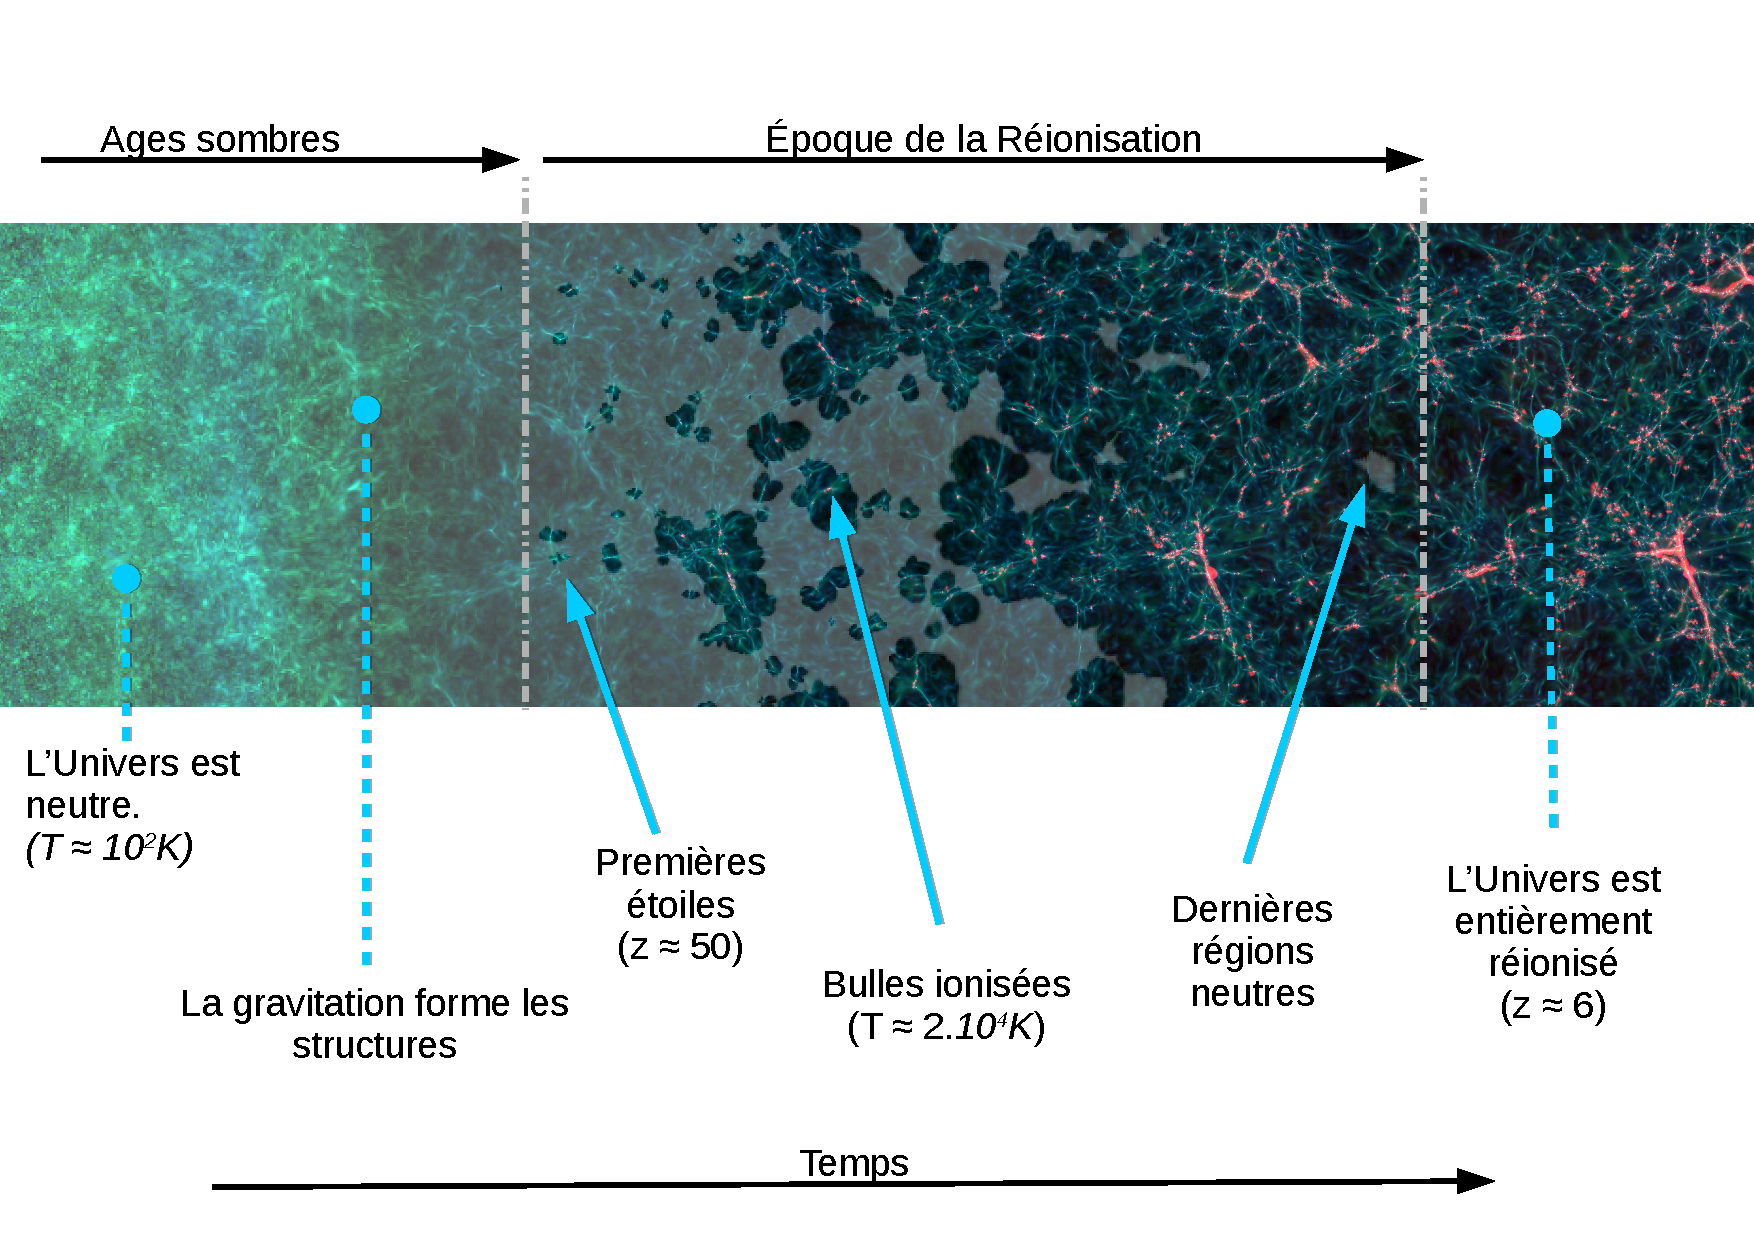
\includegraphics[width=\textwidth]{img/01/frise_legend.pdf} 
        \caption[Présentation de l'EoR]{Présentation de l'Époque de Réionisation. 
        L'apparition des premières étoiles introduit un rayonnement UV qui va petit à petit réioniser l'Univers}
 		\label{fig:frise}
\end{figure}


Nous avons vu dans le chapitre précédent que lors de la recombinaison, l'Univers est passé d'un état globalement ionisé à un état globalement neutre.
%De cette transition, qui a eu lieu a environ 380000 ans après le Bigbang, en a résulté L’émission du CMB.
Suite a cette étape, l'Univers était alors très homogène et ne disposait pas de source lumineuse, c'était les "ages sombres".
Sa dynamique était régie essentiellement par la lutte entre l'expansion et la gravitation et la compétition entre ces deux forces couplée à de très légères perturbations a menée à l'effondrement de certaines de ses parties.
Il faudra alors attendre plusieurs centaines de million d'années pour voir apparaître des surdensité de gaz suffisamment compactes pour former les première étoiles.
Ces premières sources lumineuses ont émis un puissant rayonnement ionisant qui a à nouveau séparé les protons et les électron formé lors de la recombinaison.
Il a fallut encore plusieurs centaine de million d'années pour que les première sources de rayonnement soient suffisamment nombreuses pour que leurs photons remplissent l'univers, et le fasse passer d'un état majoritairement neutre, à un état à nouveau majoritairement ionisé. 
Cette transition s'appelle l’époque de la réionisation (voir figure \ref{fig:frise}).

L'objectif de cette section est de présenter les grandes lignes des principes physique qui ont eu lieu durant cette période.
Je présenterai également quelques unes des preuve observationnelles qui confirme que la réionisation a bien eu lieu.

%à l'apparition des premières des premières étoiles.
%L'Univers va alors subir un changement d'état majeur, puisque le rayonnement énergétique des premières étoiles va de nouveau ioniser le gaz.
%C'est l'époque de la réionisation.

%Du fait que l'univers était neutre, le rayonnement n’était pas en mesure de se propager librement.
%A la suite de l'émission du fond diffus cosmologique, commence une période appelée "les ages sombres".
%L'Univers est alors composé de gaz froid soumis principalement à deux forces : la gravité et l'expansion de l'Univers.
%Ces étoiles ont émis du rayonnement suffisamment énergétique pour arracher les électrons du gaz environnant.

%Dans cette section, je vais présenter quelques unes des preuve observationnelles de la réionisation. 


\section{Influence de la réionisation sur la formation des galaxies}

Nous avons vu dans la partie dédiée au fond diffus cosmologique que lors de l'émission du \ac{CMB} l'univers n'était pas parfaitement homogène.
La croissance de ces perturbations primordiales va mener, sous l'effet de la lutte entre l'expansion et la gravitation, à un effondrement de la matière sur elle même à différents endroits.
C'est dans ces surdensités locales que vont se former les premières galaxies.

Pour qu'une surdensité s'effondre, il faut que sa masse soit supérieure à la masse de Jeans et cette masse évolue en fonction du redshift \citep{2016PhR...645....1B} : 

\begin{equation}
M_j \approx 6 \cdot 10 ^3 \left( \frac{1+z}{10} \right)^{3/2} M_\odot
\end{equation}

Lors de son effondrement, le gaz est soumis à une compression : sa température et sa pression augmente en s'opposant à la contraction.
L'effondrement des structures est alors limité et le refroidissement doit être efficace pour pouvoir continuer à effondrer le gaz (voir eg \cite{2004ARA&A..42...79B}).
Pour être en mesure de former des étoiles, un nuage de gaz doit avoir un temps dynamique :
\begin{equation}
t_{dyn} =\sqrt{\frac{3 \pi}{32 G \rho}},
\end{equation}
plus important que son temps caractéristique de refroidissement :
\begin{equation}
t_{cool} = \frac{3 nkT}{2 \Lambda(n,T)}.
\end{equation}

Dans notre cas, le taux de refroidissement $\Lambda(n,T)$ est gouverné par l'émission de rayonnement d l'hydrogène atomique ou de l'hydrogène moléculaire (voir figure \ref{fig:refroidissement}).
Ces rayonnements permettent de dissiper suffisamment d'énergie pour que l'effondrement puisse se poursuivre \citep{2001PhR...349..125B}.

\begin{figure}
        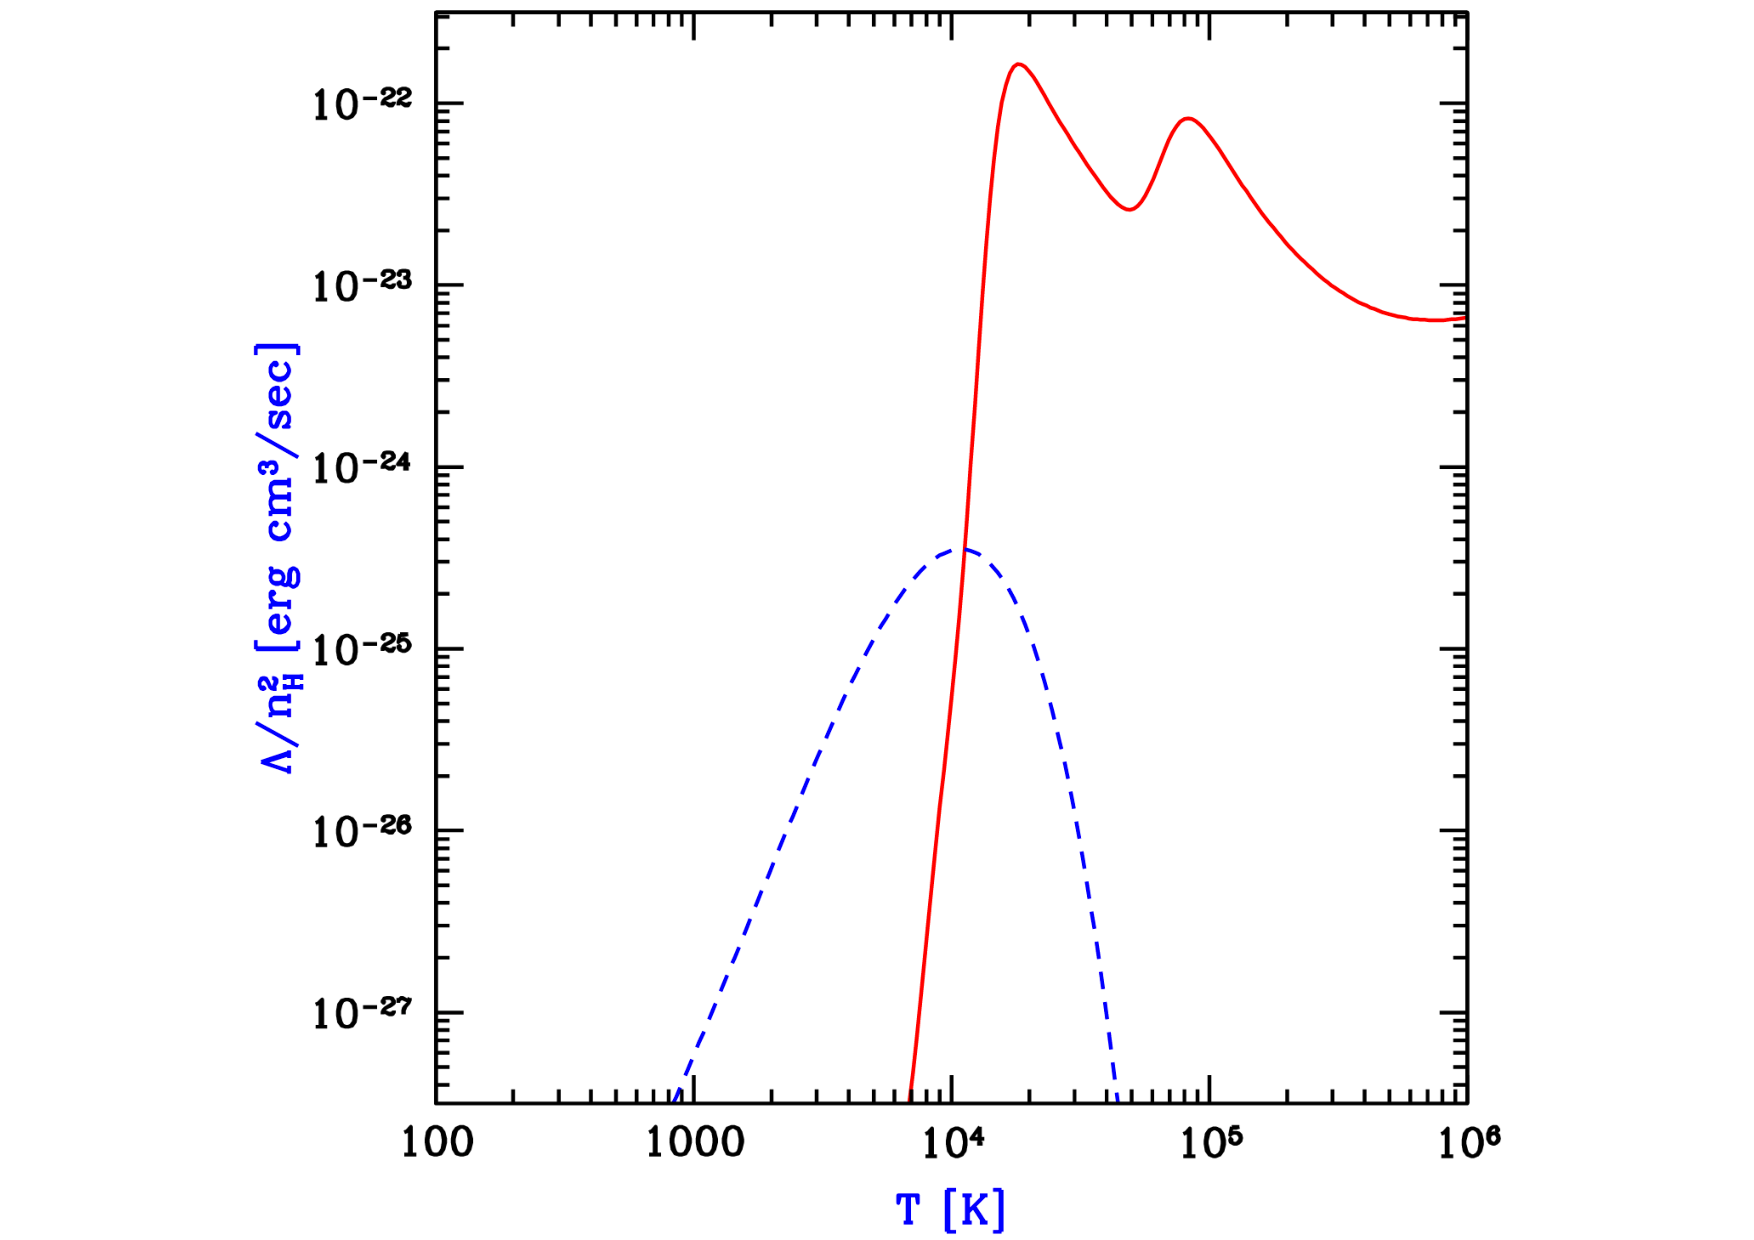
\includegraphics[width=.95\linewidth]{img/01/fonction_refroidissement.pdf} 
        \caption[Fonction de refroidissement]{Taux de refroidissement de l'hydrogène et de l'hélium atomique en rouge et moléculaire en bleu. 
        Figure extraite de \cite{2016PhR...645....1B}.
 		\label{fig:refroidissement}}
\end{figure}

Le type de processus de refroidissement majoritaire va conditionner le type du halo \citep{2002Sci...295...93A}) : on distinguera les halos à refroidissement atomiques, des halos à refroidissement moléculaire.

Les halos à refroidissement moléculaire seront appelé "mini halo" du fait de leur faible masse $M < 10^8 M_\odot$.
La formation stellaire dans ces halos est gouverné par la formation de $H_2$, or cette molécule est très sensible au rayonnement émis par les première générations d'étoiles.

Les halos à refroidissement atomique aurons une masse plus importante $M > 10^8 M_\odot$.
On distinguera cependant deux sous catégories : les halos massifs $M > 10^9 M_\odot$ et les halos de faible masse $M< 10^9 M_\odot$.
Ces dernier sont sensibles au photo-chauffage induit par le rayonnement UV \citep{1998ApJ...497...21M}.
Ces halos, voyant leur température augmenté vont également subir une augmentation de leur masse de Jeans.
L'effondrement ne sera alors plus possible et la formation stellaire stoppée.




\clearpage
\section{Principe général}

Lorsqu'une étoile se forme dans un environnement d'hydrogène neutre, son rayonnement va être capable d'ioniser l'hydrogène autour d'elle dans une zone définie.
Ces zones forment des bulles, et quand plusieurs bulles apparaissent proches les unes des autre, elles percolent pour en former une plus grande.
Ces région sont nommées régions HII et une grande partie de l'étude de l'époque de réionisation consiste à étudier leurs croissance.
Dans le but d’appréhender les principes de base à l’œuvre pendant la réionisation, nous allons commencer par nous placer dans un cas simple et idéal.

\subsection{Sphère de Strömgren}
\label{sec:stromgren}

Une source lumineuse ponctuelle apparaît instantanément dans un milieu infini, avec une densité et une température homogène et composé exclusivement d’hydrogène neutre.
Les questions sont alors : 
\begin{itemize}
\item Comment va évoluer l’état d'ionisation du gaz autour de cette source ?
\item Quelle région cette source va ioniser autour d'elle?
\end{itemize}

En considérant l'équilibre entre $\dot{N_\gamma}$ le nombre de photons ionisant émis par la source et le taux de recombinaison du milieu, \cite{stromgren_physical_1939} a exprimé l'évolution du rayon  $r_i(t)$ de la sphère ionisée :

\begin{equation}
\frac{dr_i(t)^3}{dt} = -n_H \alpha_B(T)r_i (t)^3 + \frac{3 \dot{N_\gamma} }{4 \pi n_H},
\end{equation}

où $\alpha_B(T)$ est le coefficient de recombinaison, fonction de la température et $n_H$ la densité d'hydrogène neutre.
La solution de cette équation est de la forme :

\begin{equation}
r(t) = r_s \left( 1 - e^{-t\cdot \alpha_B(T) n_H } \right)^{1/3}
\end{equation}

%
%\begin{equation}
%t_{rec} = \left( \alpha_B(T) n_H \right) ^{-1}
%\end{equation}

Le rayon de Strömgren est défini comme étant la solution stationnaire de cette équation:

\begin{equation}
r_s = \left( \frac{3 \dot{N_\gamma} }{4 \pi \alpha_B(T) n_H^2} \right)
\end{equation}

Nous voyons ici que connaissant l'émissivité de la source et la densité et température du milieu environnant, il est possible d'estimer la taille de sa région HII.

\subsection{Le cas non idéal}
Nous venons de voir un modèle théorique sensé représenter la croissance des régions HII de manière individuelles, en réalité : 
\begin{itemize}
%\item la densité n'est pas homogène,% (motif en papillon autour des filament)
\item les sources ne sont pas isolées,
\item l'intensité des sources n'est pas constante. %Les étoiles évoluent et meurent, si il n'y a 
\end{itemize}

Pour estimer l'évolution de la fraction d'hydrogène ionisée dans l'Univers, il est nécessaire de calculer la balance entre le taux d'ionisation et le recombinaison \citep{0004-637X-514-2-648, RevModPhys.81.1405} en utilisant :
\begin{equation}
\frac{dQ_{HII}}{dt} = \frac{\dot{N}_{ion}}{ <n_H>} - \frac{Q_{HII}}{t_{rec}},
\end{equation}

où, le taux d'émission de photon ionisant $\dot{N}_{ion}= dot{n}_{ion} f_{esc}$, dépend de $dot{n}_{ion}$ le nombre de photon ionisant produit et de $f_{esc}$ la fraction d'échappement des photons. elle caractérise le lien entre les photon ionisant produit par les sources et les photons qui vont être effectivement utiles à ioniser l'\ac{IGM}.
Il est possible de mettre des contraintes sur le taux de photo-ionisation (voir figure \ref{fig:photoionisationrate}).

%$ <n_H>$ est la densité moyenne d'Hydrogène dans l'Univers, comme il dépend de $a$, ce terme contient l'information de l'expansion de l'Univers.
%Le second terme est le terme de recombinaison, $t_{rec}$

\begin{figure}
        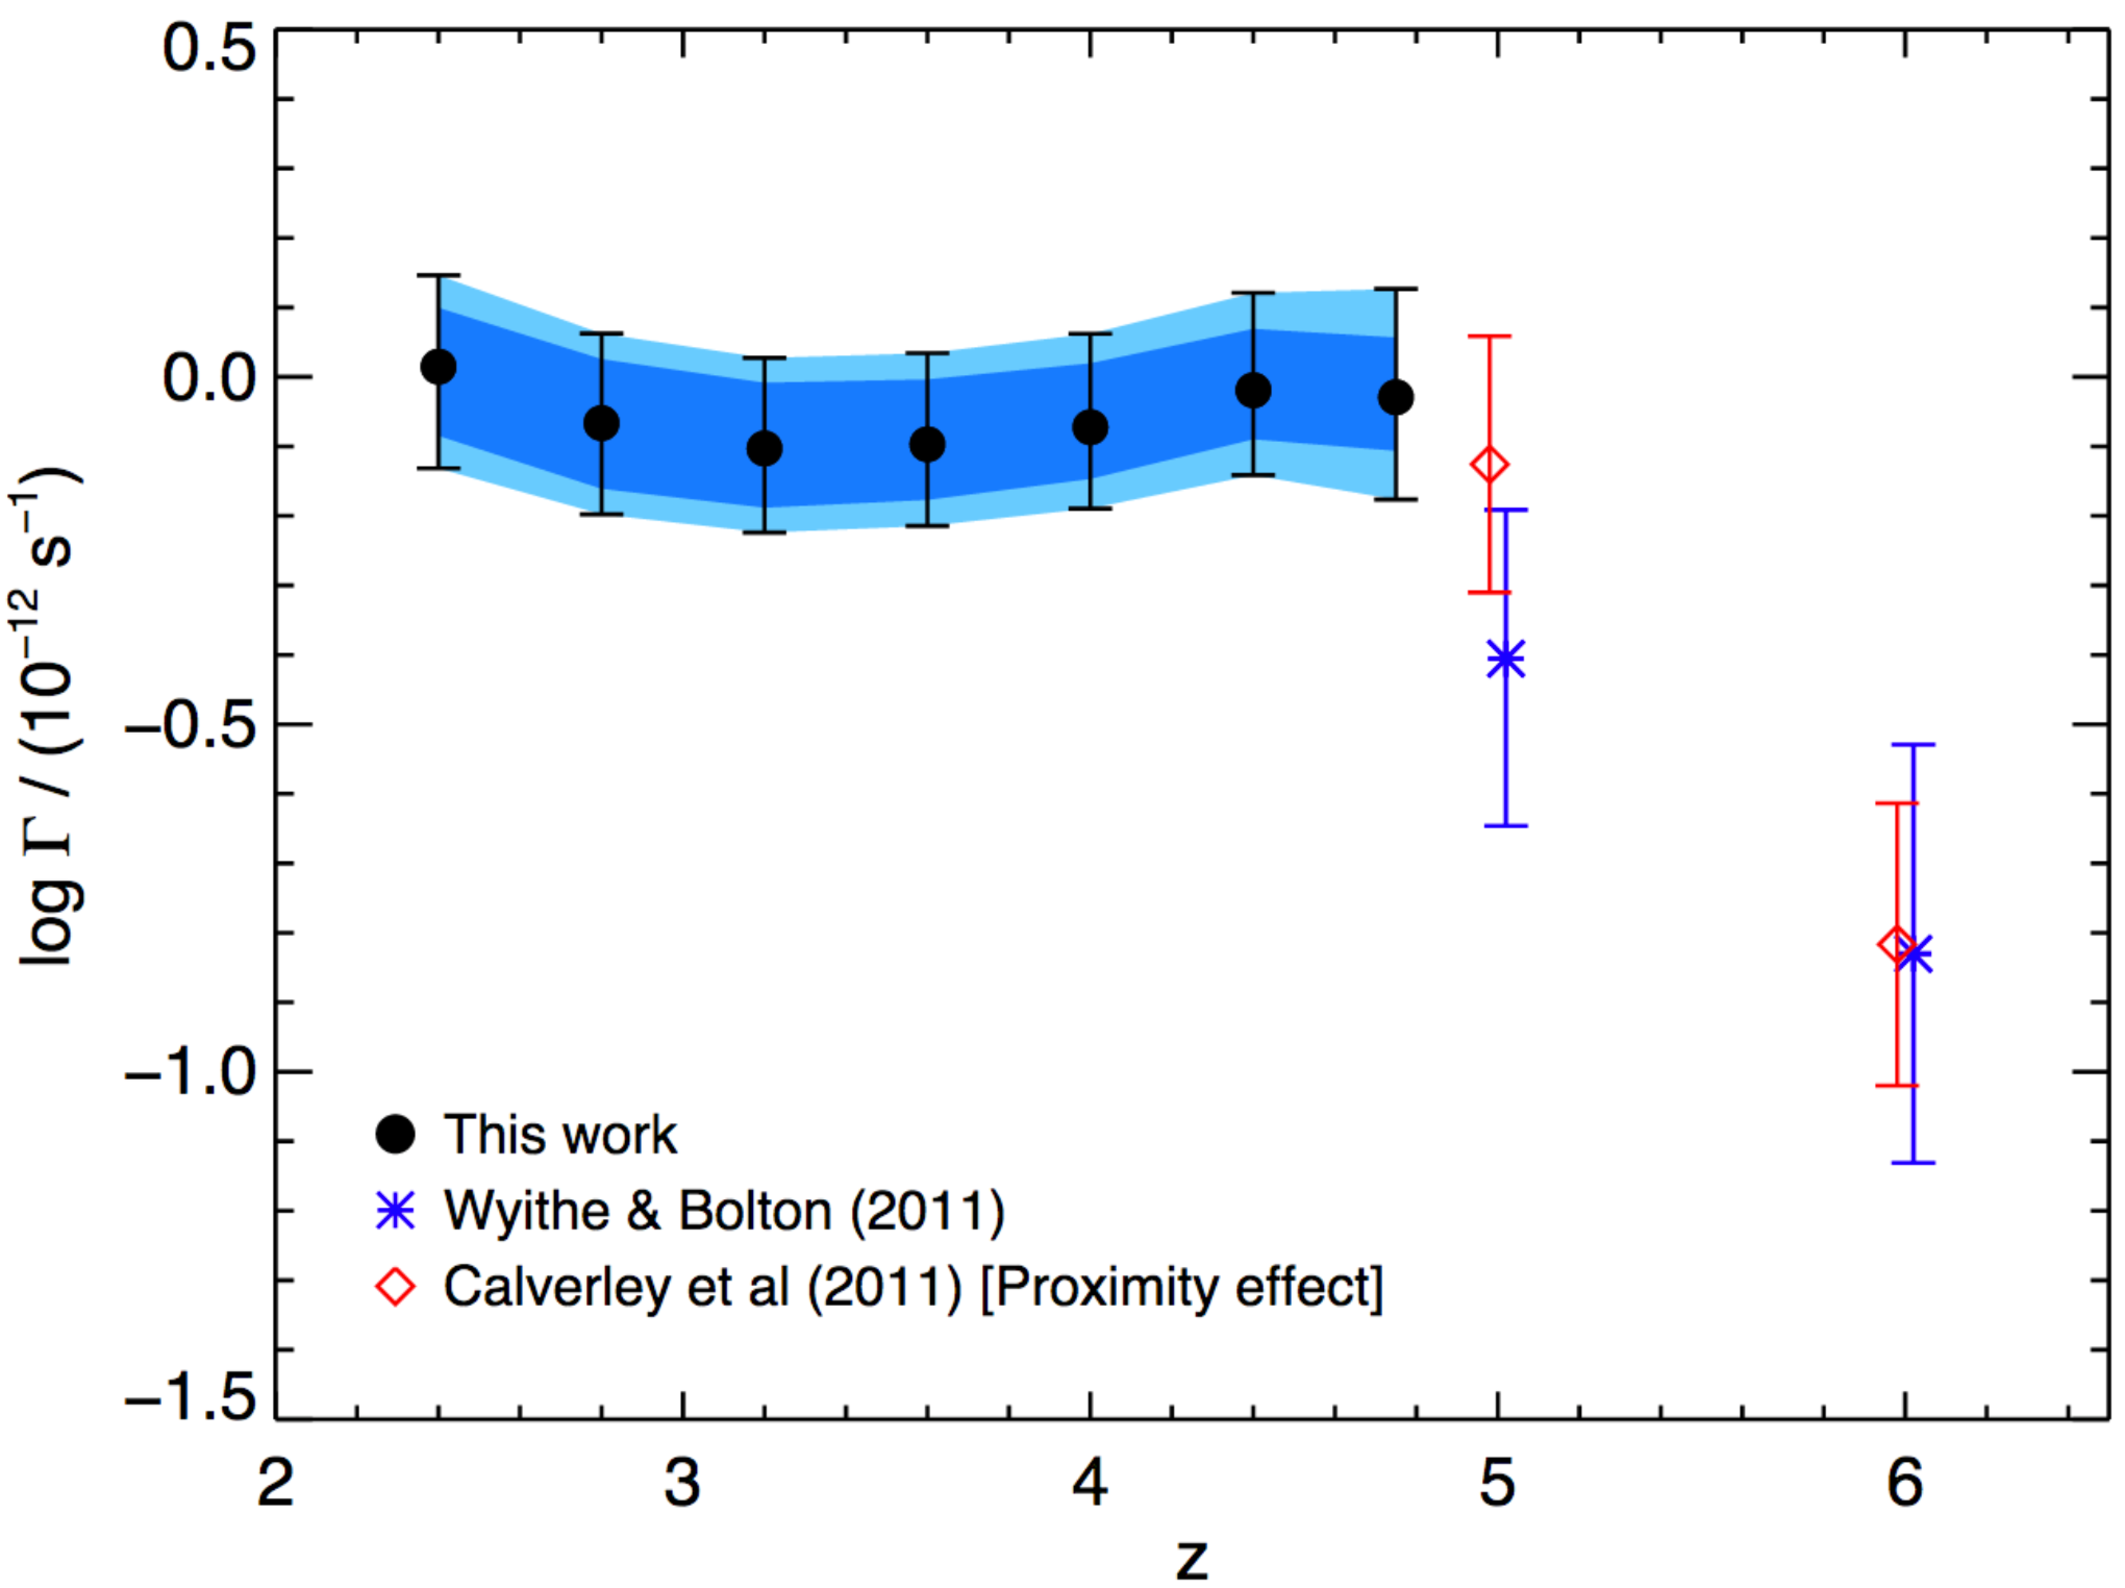
\includegraphics[width=.95\linewidth]{img/01/photon_obs.pdf} 
        \caption[Taux de photo-ionisation ]{Taux de photo-ionisation de l'\ac{IGM}. 
        Figure extraite de \cite{2013MNRAS.436.1023B}.
 		\label{fig:photoionisationrate}}
\end{figure}



%taux d'effondrement des structures.

%l'Univers de réionise en entier car les sources sont nombreuses et c'est la percolation des régions HII des régions successives d'étoiles 

%Les régions HII croissent de manière asymétrique en fonction de la géométrie du milieu, et forment des motifs en "papillons" autour des amas et des filaments.
%La percolation de ces régions augmente petit à petit la fraction ionisée de l'Univers, jusqu'à ce qu'il ne reste plus que une fraction de neutre de l'ordre de $1-Q_{HII}=10^{-4}$.

Le taux de production des photons est fonction du taux de formation stellaire.
La figure \ref{fig:obs} présente les fonctions de luminosités des galaxies à haut redshift ainsi que les contraintes déterminées à partir de celles ci sur le taux de formation stellaire
Se sont les générations successives d'étoiles et l'augmentation du taux de formation stellaire qui permet a l'Univers de réioniser en entier.

\begin{figure}
		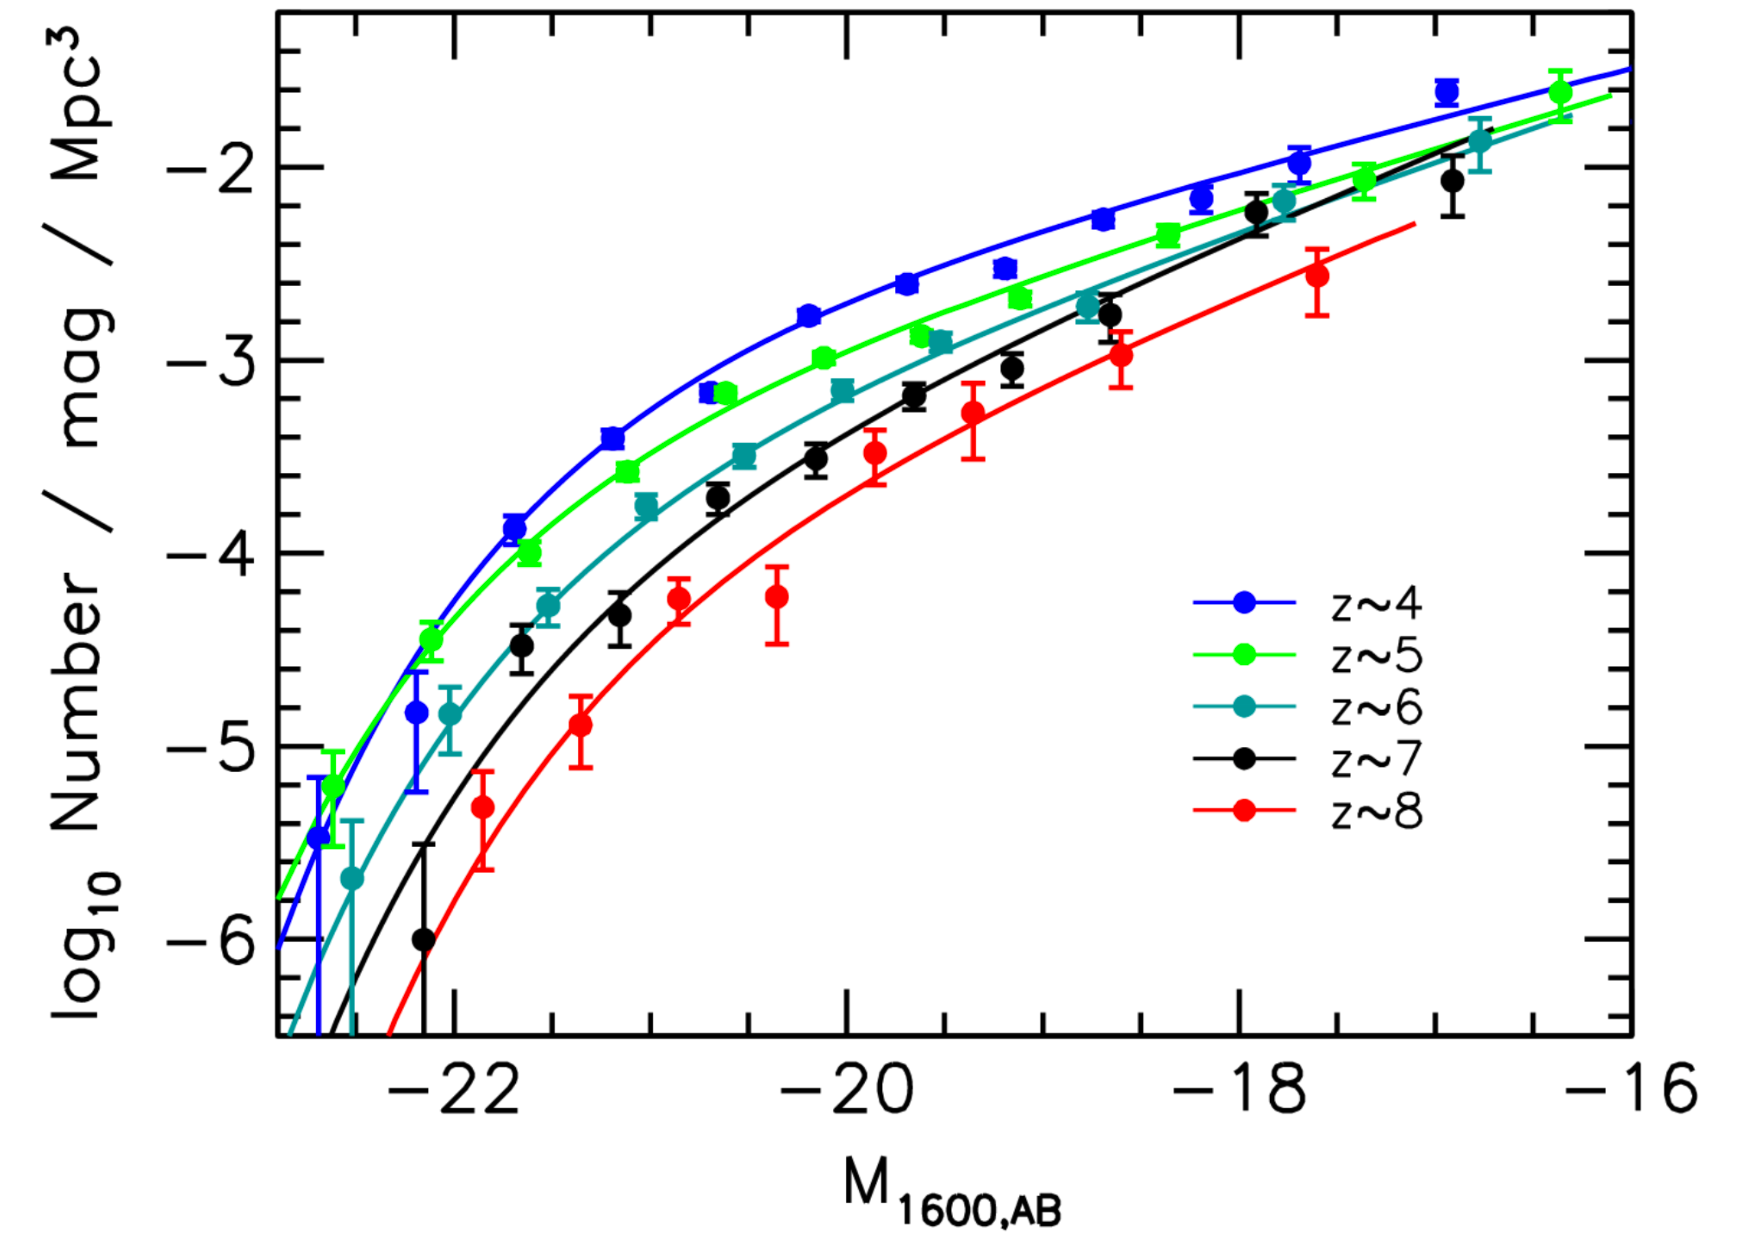
\includegraphics[width=.95\linewidth]{img/01/UV_lum_obs.pdf} 
        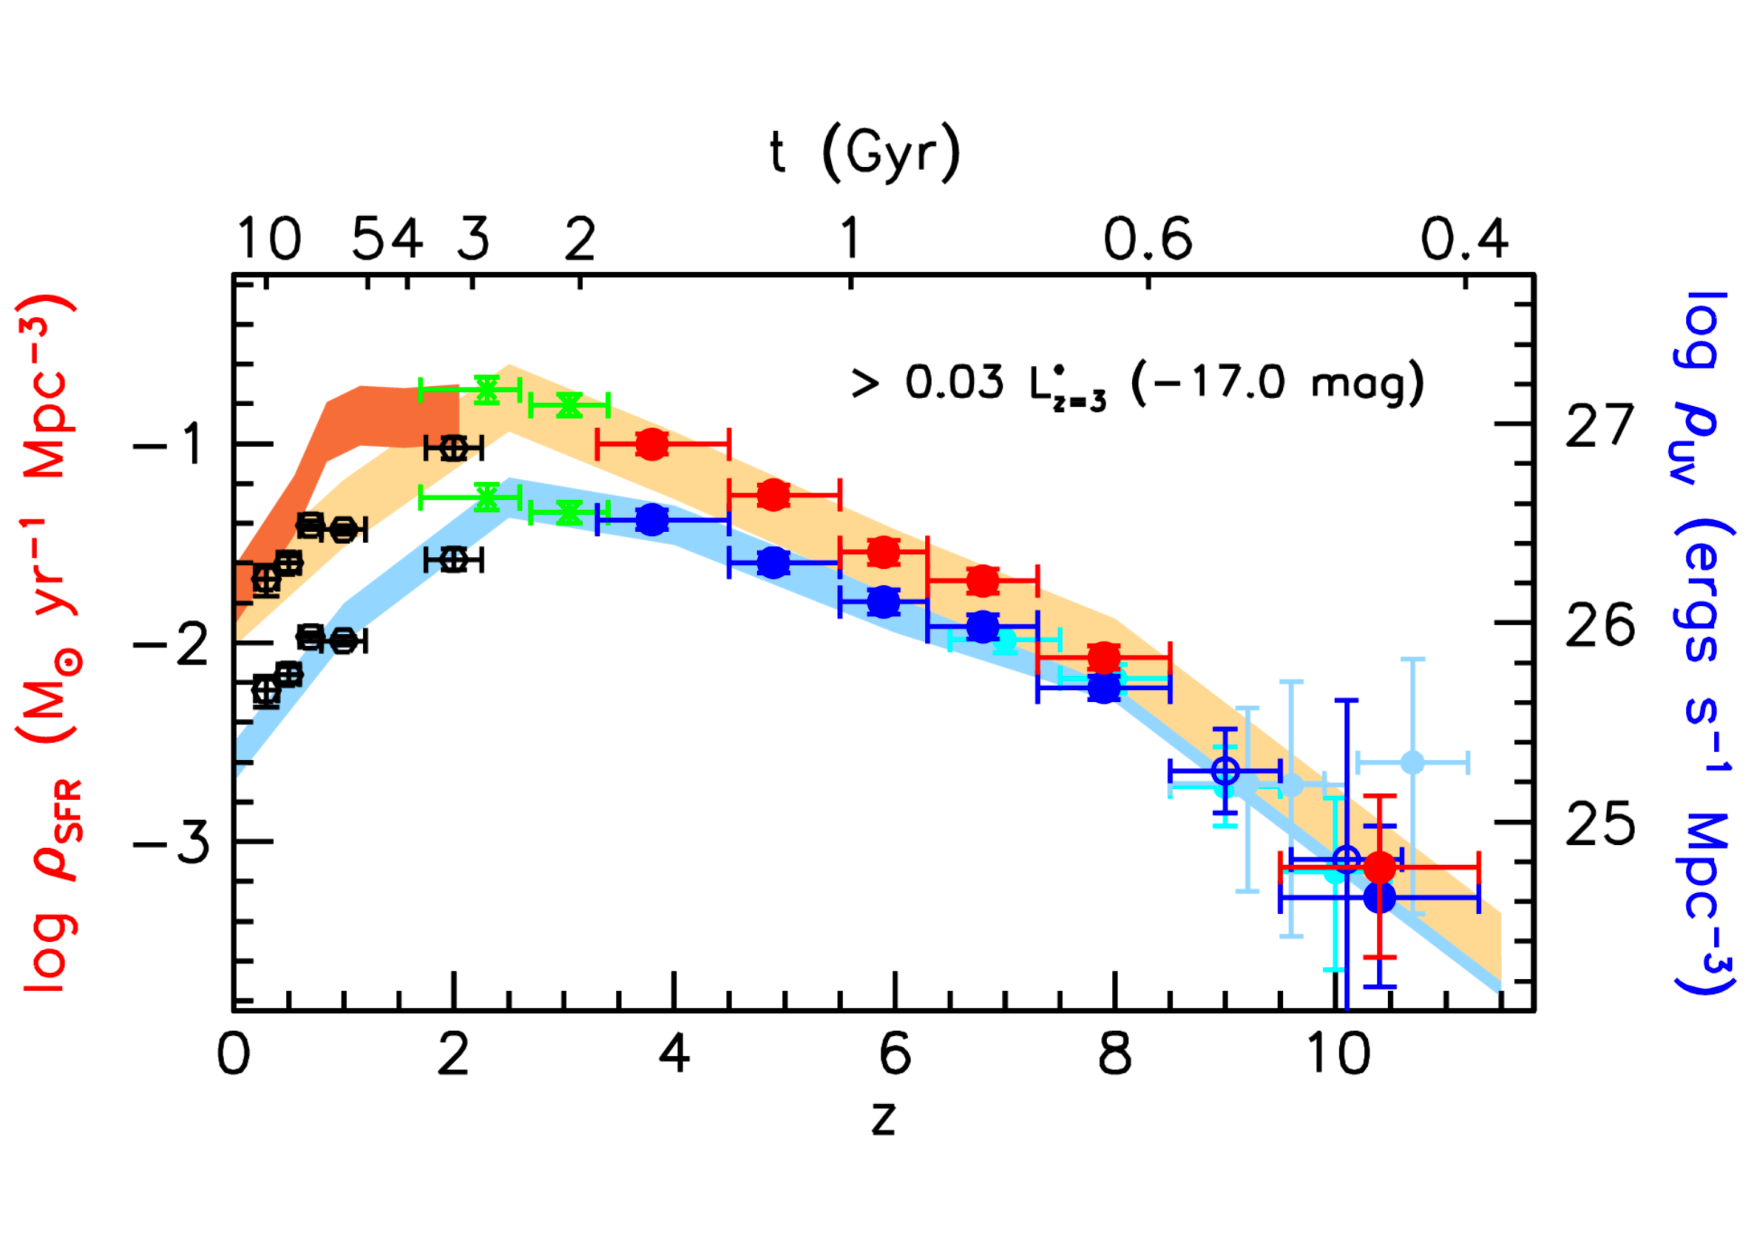
\includegraphics[width=.95\linewidth]{img/01/SFR_obs.pdf} 
        \caption[Contrainte SFH]{Haut: fonction de luminosité à haut redshift. 
        Bas : contraintes observationnelle sur l'histoire de formation stellaire à haut redshift dérivé des fonctions de luminosités. 
        Figures extraites de \cite{bouwens_reionization_2015}.
 		\label{fig:obs}}
\end{figure}

Le taux de production des photons est aussi fonction du profile d'émissivité des sources.
Ce profil d'emmissivité sera dépendant entre autre de la fonction de masse initiale


\clearpage
\section{Preuves observationnelles}
\label{sec_contraintes_obs}

Dans cette section nous verrons quelles sont les principales observations montrant que la réionisation a effectivement eu lieu.

\subsection{Spectre de quasar et épaisseur optique Lyman alpha}

Historiquement, les spectres de quasar lointains ont été les premières preuves que l'Univers était fortement neutre dans le passé.
Les quasars sont des objets suffisamment brillants pour être observé à très grandes distance.
\cite{1965ApJ...141.1295S} observe que le spectre des plus lointains d'entre eux présente une absorption caractéristique.%, appelée tunel Gun-Peterson \citep{1965ApJ...142.1633G}.
Avant de poursuivre, il est nécessaire  de revenir sur le spectre d’émission de l’hydrogène.

\subsubsection*{Raie Lyman alpha}

%\begin{figure}
%\centering
%        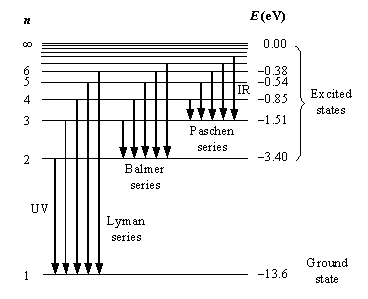
\includegraphics[width=.9\textwidth]{img/01/lyman.jpg} 
%        \caption[Raies de l'hydrogène]{Changement de niveau d'énergie de l'atome d'hydrogène}
% 		\label{fig:lyman}
%\end{figure}
%(cf Fig. \ref{fig:lyman}) 

La série de Lyman correspond a la transition atomique menant au fondamental de l'atome d'hydrogène.
Il existe plusieurs série de transition autre que celle de Lyman mais cette dernière est la plus énergétique et la plus fréquente, et donc la plus facile à détecter.
Il y a émission d'un photon Lyman-alpha pendant la transition de l'électron du premier état excité vers l’état fondamental (n2 -> n1).
L'énergie de cette transition est de 1216 $\AA$,  ce qui place l’émission dans l'Ultra Violet.
Réciproquement, la transition n1 vers n2 mène a l'absorption d'un photon Lyman-alpha.
C'est a dire que si un nuage de gaz neutre se trouve entre une source et l'observateur, le spectre réceptionné présentera une raie d'absorption à 1216 $\AA$.

\subsubsection*{Forêt Lyman alpha}

Maintenant considéreront des distances cosmologiques entre la source et l'observateur.
Durant le parcours des photon, l'Univers aura subi une expansion et le spectre d'émission de la source sera décalé vers le rouge.
Le spectre présentera des raie d’absorption à différents endroits suivant le moment de rencontre des différents nuages de gaz neutre.
C'est série de raies est très dense à haut redshift et est appelée forêt Lyman alpha.

\subsubsection*{Tunnel Gunn-Peterson}

Si nous considérons maintenant que la source est a l’intérieur d'une zone neutre, la série de raies absorbée ne sera plus discrète mais continue.
C'est ce continuum d’absorption que l'on nomme tunnel Gunn-Peterson \cite{1965ApJ...141.1295S}
La figure \ref{fig:spectre_quasar} montre une série d'observations de spectres de quasars.
Ces spectres sont classés par redshift, et le tunnel Gunn-Peterson des plus éloignés est particulièrement visible.

%Dans le cas de la reionisation, les sources sont des quasar.
%Les quasars sont des objets suffisamment brillants pour être observé a très grandes distance.
%Il est observé que plus leur redshift est important, plus leur foret lyman alpha est important.
%Les plus lointains d'entre eux présentent  un tunnel gun peterson.

\begin{figure}
        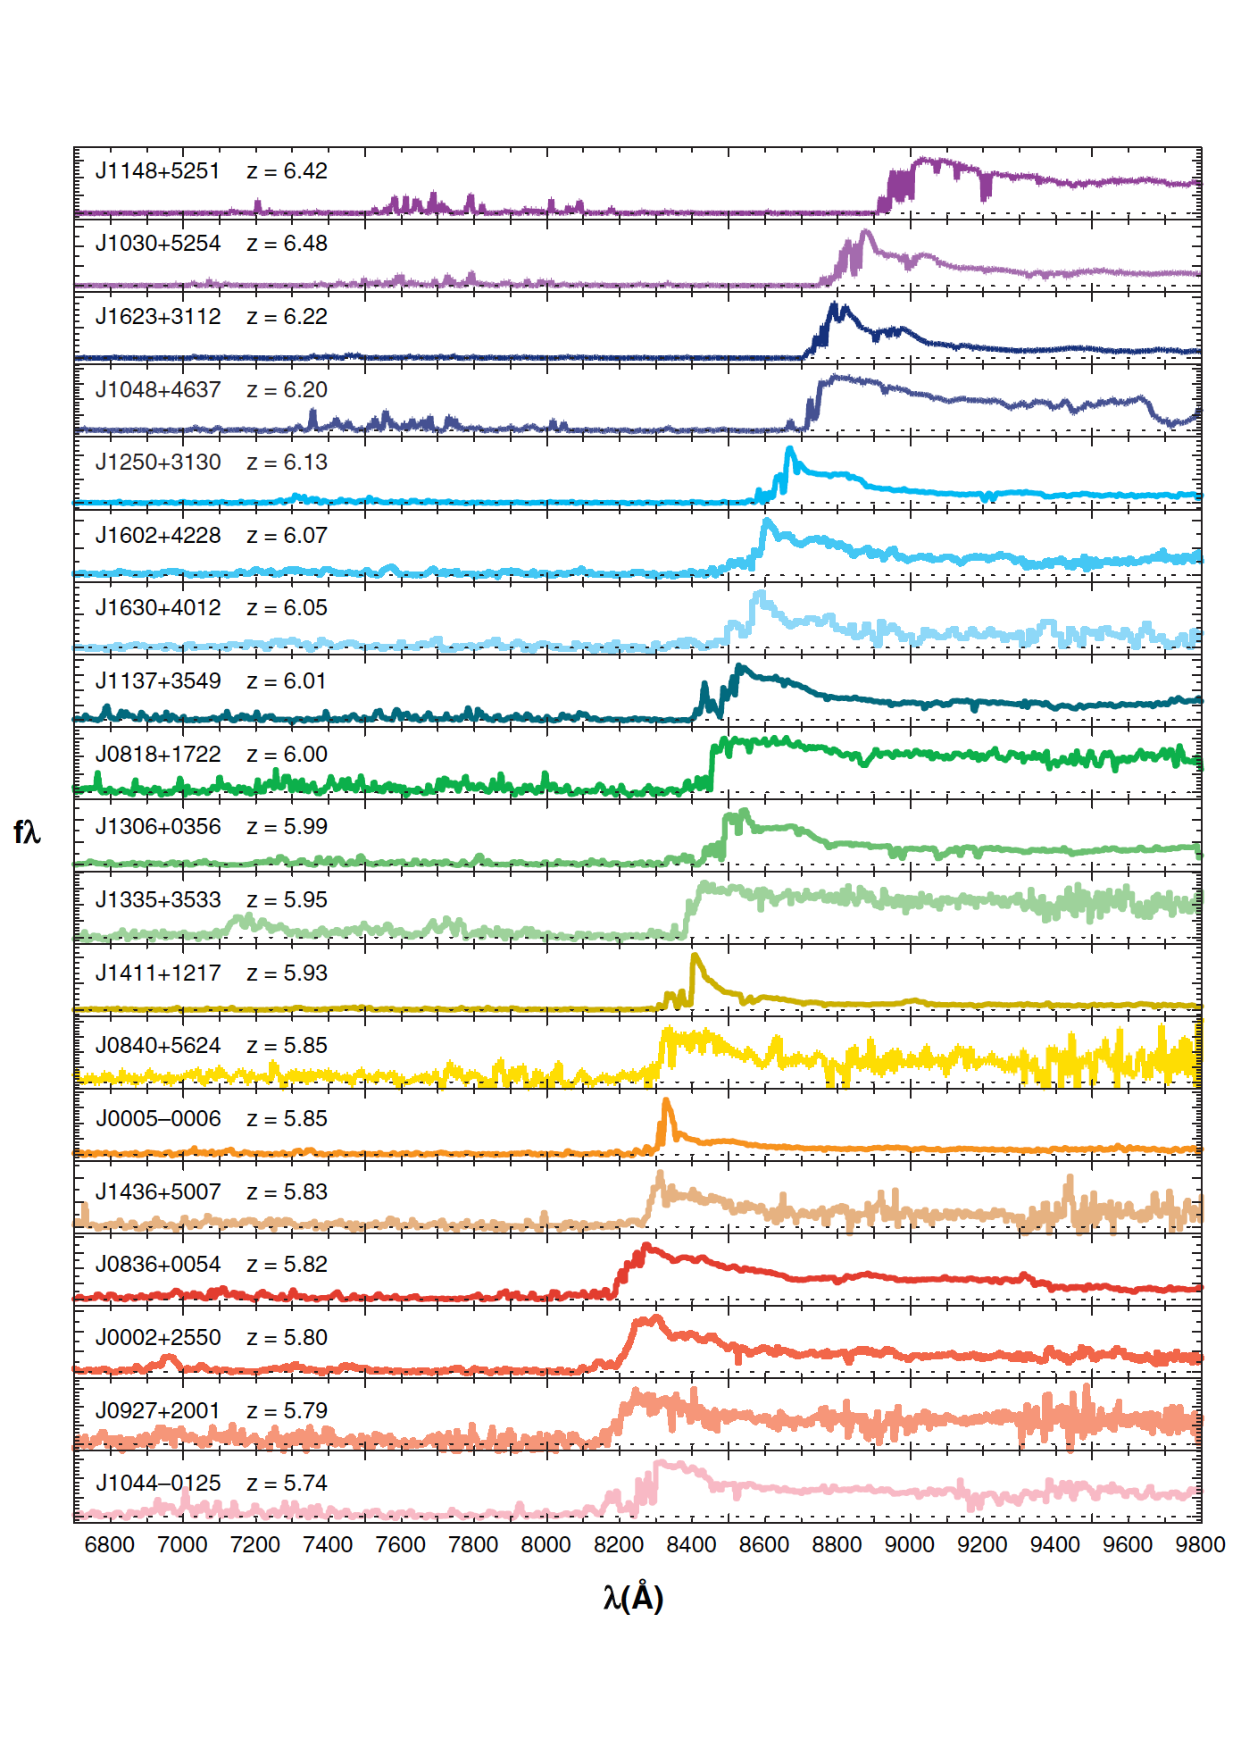
\includegraphics[width=.95\linewidth]{img/01/quasar_spectre.pdf} 
        \caption[Spectre de quasars]{Spectre de quasars à différents redshift présentant un tunnel Gunn Peterson.
		Image extraite de \cite{fan_constraining_2006}.
 		\label{fig:spectre_quasar}}
\end{figure}

\subsubsection{Épaisseur optique}

A partir des spectres obtenu il est possible de mesurer l’épaisseur optique traversée par les photons Lyman alpha à l'aide de la formule suivante:
\begin{equation}
\tau_{GP} = \frac{\pi e^2}{m_e c} f_\alpha \lambda_\alpha H^{-1}(z) n_{HI},
\end{equation}
où $f_\alpha$ est la force d'oscillateur de la transition Lyman alpha, $\lambda_\alpha = 1216 \AA$, $H(z)$ est la constante de Hubble, $n_{HI}$ la densité d'hydrogène neutre.

En appliquant cette formule aux différents spectres observés (figure \ref{fig:spectre_quasar}), \cite{fan_constraining_2006} ont mesuré la variation d'épaisseur optique en fonction du redshift.
Les résultats sont présentés sur la figure \ref{fig:epaisseur_optique_quasar}.
Il apparaît clairement que l'épaisseur optique augmente avec le redshift.

\begin{figure}
        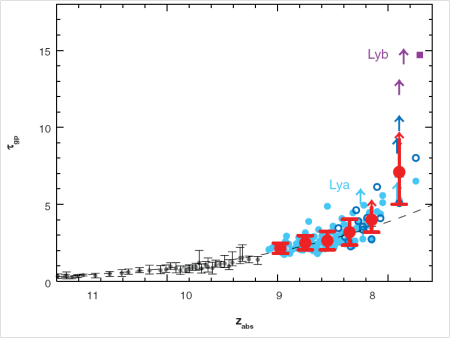
\includegraphics[width=.95\linewidth]{img/01/epaisseur_optique_quasar.png} 
        \caption[Epaisseur optique Lyman alpha]{%https://ism2009.wordpress.com/2009/04/28/on-the-density-of-neutral-hydrogen-in-intergalactic-space/
		Épaisseur optique calculée a partir des spectres de quasar de la Fig\,\ref{fig:spectre_quasar}
        Image extraite de \cite{fan_constraining_2006}.}
 		\label{fig:epaisseur_optique_quasar}
\end{figure}

\subsubsection{Les contraintes sur l'état d'ionisation}

A partir de l'épaisseur optique, il est possible de déterminer la fraction d'hydrogène neutre traversée.
Une compilation des contraintes sur la fraction d'hydrogène neutre a été réalisé par \cite{2015ApJ...811..140B} et est présenté sur la figure \ref{fig:compile_constrains}.
On y observe un brusque changement à redshift $z\approx6$.
Cette chute dans la fraction de neutre représente la fin de la période de réionisation.

\begin{figure}
        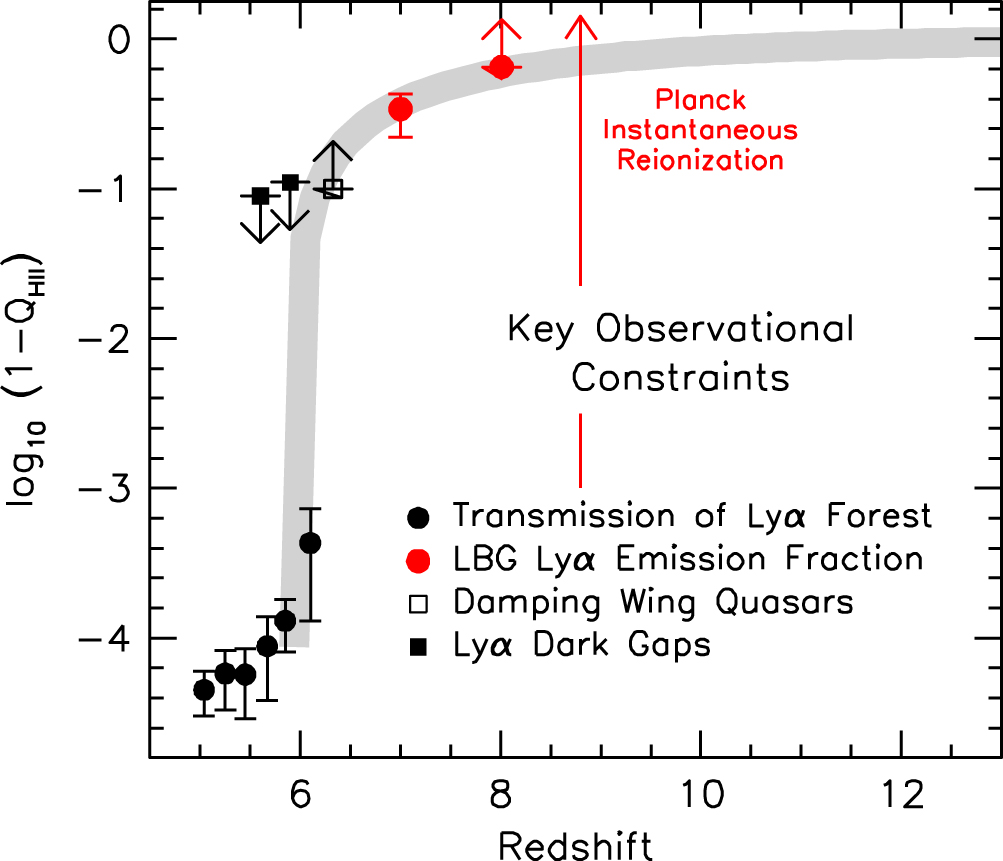
\includegraphics[width=.95\linewidth]{img/01/xionconstrains.jpg} 
        \caption[Fraction de neutre]{Fraction de neutre en fonction du redshift a partir d'observation lymann alpha.
        Compilation par \cite{2015ApJ...811..140B}}
 		\label{fig:compile_constrains}
\end{figure}


\subsection{CMB et épaisseur optique Thomson}

Une observation de la réionisation se trouve également dans les photons CMB, car la réionisation constitue un avant plan qui les a influencé. 
Les photons émis lors de la recombinaisons ont été diffusé, par le grand nombre d'électron libérer pendant la réionisation.
Cette succession de diffusions Thomson, se traduit par une épaisseur optique qui prend la forme : 

\begin{equation}
\tau_z = c \sigma_t \int_z^0 n_e (z) \frac{dt}{dz} dz,
\end{equation}
avec $\sigma_t$ la section efficace Thomson et $n_e (z)$ la densité d'électron libre.

L'épaisseur optique Thomson cesse d'augmenter à partir d'un certain redshift du à l’absence d'électrons libres permettant les diffusions.
Une représentation de cette contrainte, observée par le satellite Planck se trouve sur la figure \ref{fig:epaisseur_optique_thomson}.
Différent modèles réionisation y sont également présentés.
En utilisant un modèle de réionisation instantané, \cite{planck_collaboration_planck_2016} estime le redshift de réionisation à $z_r = 8.8 ^{+1.3}_{-1.2}$.

\begin{figure}
        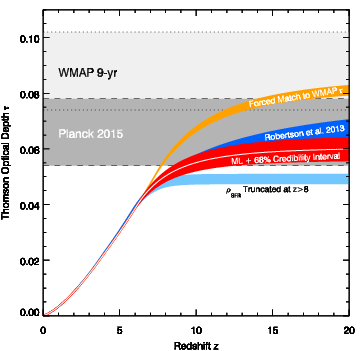
\includegraphics[width=.9\linewidth]{img/01/epaisseur_optique_thomson.png} 
        \caption[Epaisseur optique Thomson]{%https://inspirehep.net/record/1343310/plots
		Contrainte sur l'épaisseur optique Thomson.
        Image extraite de \cite{2015ApJ...802L..19R}
 		\label{fig:epaisseur_optique_thomson} }
\end{figure}

\subsection{Ligne 21 cm et observations}


Une raie a 21 cm est émisse par les nuages d'hydrogène neutre.
Lorsque que le spin de l'électron et du proton sont opposée, le niveau d'énergie de l'atome est légèrement supérieur au cas ou les spins sont alignés.
Ces deux niveaux ont des énergies très proches et la transition est dite hyperfine.


Une des difficultés de l’étude de la période de réionisation est que celle si a eu lieu tôt dans l'histoire de l'univers lors de son premier milliard d'années.
Cette distance temporelle impose de regarder loin spatialement et donc de disposer de moyen observationnels important.
Nous somme au balbutiement des observation de la réionisation et une série de missions dédiées a l'observation de la raie 21cm vont venir livrer leurs résultats et compléter notre compréhension de la réionisation dans les années à venir :
\begin{itemize}
\item SKA (Square-Kilometer Array) \href{https://skatelescope.org/}{site}
\item LOFAR (Low Frequency Array) \href{http://www.lofar.org/}{site}
\item HERA (Hydrogen Epoch of Reionization Array) \href{http://reionization.org/}{site}
\end{itemize}
%


%Lors du changement de spin d'un électron 
%
%\subsection{polarisation du CMB)}
%
%\subsection{fonction de luminosité UV}

%\section{Les futures observations}
%\subsection{SKA}
%\subsection{LOFAR}


\section{Quelques questions en suspens}

%quand est ce arrivé?
%quelles sont les sources? -> débat galaxies vs quasars

%En utilisant la halo mass function presenté en TODO REF, 

La provenance des photons qui ont réionisé l'Univers est toujours indéterminée.
En étudiant la répartition du nombre de galaxies en fonction de leurs masses, on observe que les galaxies les moins massives sont nombreuse et que les galaxies les plus massives sont rare.
Or, plus une galaxie est massive, plus celle ci va créer des étoiles, et donc eméttres des photons.
La balance entre les nombreuses galaxies peu lumineuses, et les rare galaxies extrêmement lumineuse reste à déterminer.

De plus, les quasars, objets extrêmement lumineux, situé dans les galaxies les plus massives, augmente encore le budget de photon.
Les quasars ont contribué à réioniser l'Univers mais dans quelles proportion?
La figure \ref{fig:gal_AGN} présente le budget de photon plausible pour les galaxies ou les quasars selon \cite{trac_computer_2011}.
Il faut un certain temps pour mettre en place les conditions propices à l'apparition d'un quasar, est ce que ce temps a été suffisant avant z=6, pour en former suffisamment ?
Certain travaux soutiennent que c'est le cas (eg \cite{chardin_large-scale_2017}) cependant seul le rayonnement provenant des galaxies a été considérer lors de cette thèse.

Si ce sont les galaxies qui ont réionisé l'Univers, quelle est le ratio entre la quantité de rayonnement produite et la quantité de rayonnement capable d'atteindre l'\ac{IGM}?
La fraction d'échappement ($f_{esc}$) permet de faire le lien entre les observations et la physique réellement en place au sein des galaxies.
Elles dépend de nombreux paramètres comme la formation stellaire ou les propriétés du milieu.
Comment évolue t-elle en fonction de la masse des galaxies? 

\begin{figure}
        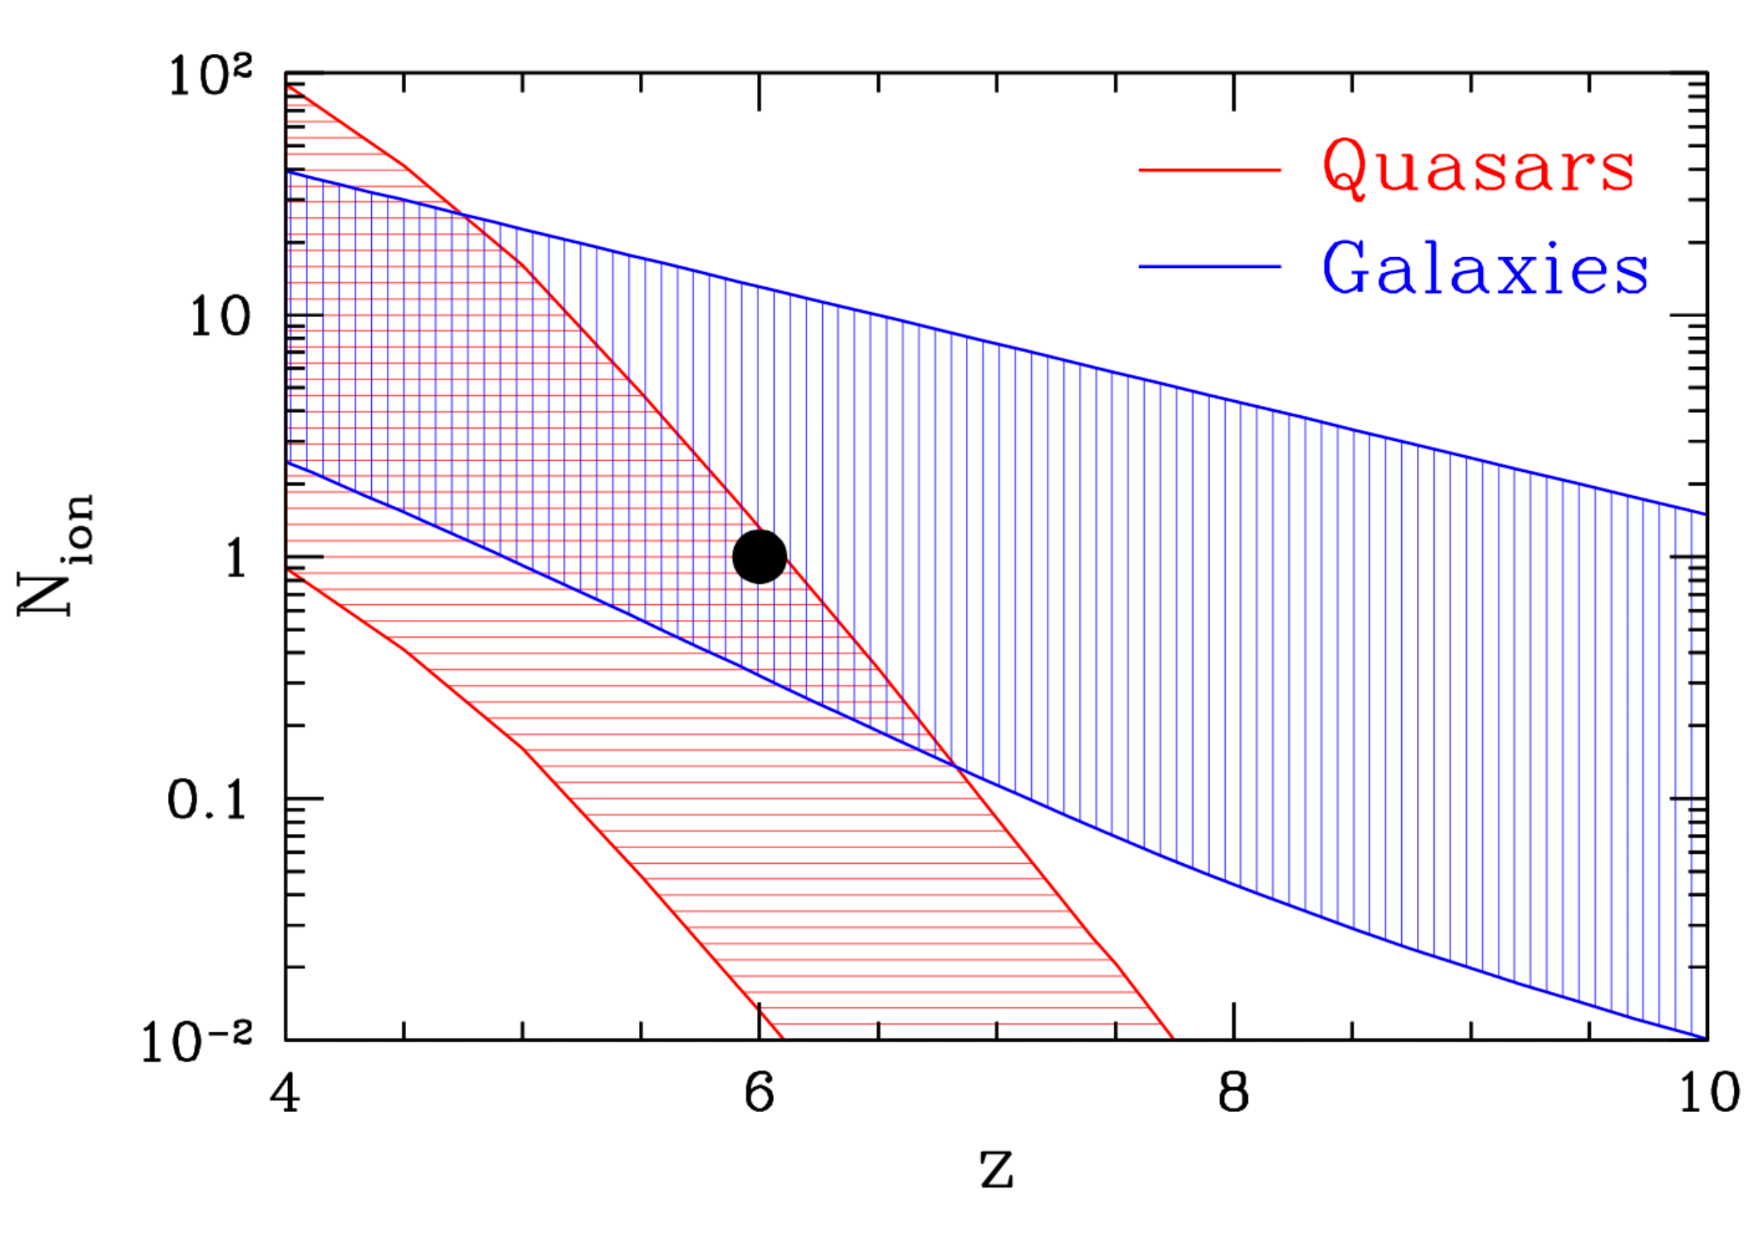
\includegraphics[width=.9\linewidth]{img/01/gal_AGN.pdf} 
        \caption{Budget de photons provenant des galaxies et des quasars durant la reionization selon \cite{trac_computer_2011}.
 		\label{fig:gal_AGN} }
\end{figure}

%outlier dans l'épaisseur optique des quasars
%Le groupe local ?
%Le développement d’expériences destinées entre
%autres le signal à 21 cm de la réionisation comme 


